\subsection{Wormhole}
\label{Wormhole}

%This seems to be made redundant by SurfaceOfRevolution.tex and PortalSpace2d.tex

In order to allow more interesting manifolds than a few that I hard code in, I have implemented connected sums of manifolds. Unfortunately, almost none of the well-known manifolds can be smoothly connected without changing their metrics. In order to facilitate this, I have found a class of manifolds that can be used as intermediates to smoothly connect two manifolds of constant curvature, and which allows geodesics to be easily calculated. I call them wormholes.

The wormhole is topologically $S^2 \times \mathbb{R}$, but with a different metric. A geodesic between two points on this metric can be found with the following method:

Given $p_1, p_2 \in S^2 \times \mathbb{R}, p_1 = (s_1,r_1),p_2 = (s_2,r_2)$ where $s_1,s_2 \in S^2, r_1,r_2 \in \mathbb{R}$.
Let $S$ be the great circle containing $s_1$, $s_2$.
The points $p_1, p_2$ are in the slice $S \times \mathbb{R}$ of $S^2 \times \mathbb{R}$.
Let $\theta_1, \theta_2 \in S$ be $s_1, s_2$ under the inverse inclusion map.
Consider $p'_1 = (\theta_1,r_1), p'_2 = (\theta_2,r_2)$.
$S \times \mathbb{R}$ corresponds to a quotient space of the half-plane model of $\mathbb{H}^2$ via $\phi:(\theta,r) \mapsto (e^{k\theta} \cos r, e^{k\theta} \sin r)$ where $k$ is a constant depending on the quotient space.
The two semicircles in figure \ref{fig:the_figure} are identified to form the quotient.

\begin{figure}[h]
\subfigure[$S^2 \times \mathbb{R}$]{
	\label{fig:S2xR}
	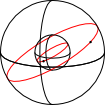
\includegraphics[scale=0.5]{../images/S2xR.png}
}
\subfigure[Half Plane]{
	\label{fig:halfplane}
	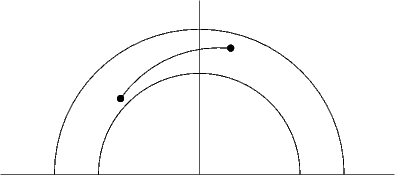
\includegraphics[scale=0.3]{../images/HalfPlane.png}
}
\subfigure[Radial Lines]{
	\label{fig:radiallines}
	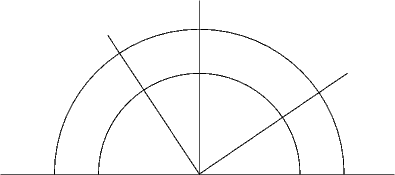
\includegraphics[scale=0.3]{../images/RadialLines.png}
}
\label{fig:the_figure}
\caption{Illustration of finding geodesics on Wormhole}
\end{figure}

Find a geodesic in $\mathbb{H}^2$ that connects $\phi(p'_1)$ and $\phi(p'_2)$, and map it back to $S \times \mathbb{R}$ and finally $S^2 \times \mathbb{R}$.

Radial lines in $\mathbb{H}^2$ are curves of constant curvature. These map to closed loops in $S \times \mathbb{R}$. The angle of the line controls how the curvature and diameter relate, allowing connection to a space of a specific curvature, such as Euclidean or hyperbolic.
